\chapter{Methods and data}
\label{sec:methods}
This chapter summarises tools and methods to analyse the numerical simulations and describes utilized measurements and data. At first, Section \ref{sec:spectral_filter} provides an overview on spectral filters applied to the simulations' output and the measurements. Then Section \ref{sec:wavelet} introduces the wavelet analysis used in Chapters \ref{sec:results3D} and \ref{sec:mf_comp} to derive horizontal and vertical wavelengths of GWs. It follows a description of measurements from a Rayleigh lidar system in Río Grande, Argentina, in Section \ref{sec:coral} and a short comment on used ERA5 data in Section \ref{sec:era5}.

% This is particularly useful for measurements,
\section{Spectral filters}
\label{sec:spectral_filter}
Spectral filters are applied for smoothing quadratic quantities like momentum and energy fluxes and for separating quantities like temperature into perturbations and a background state. Both applications utilize lowpass filters in the spatial domain. Temporal filtering is not used.

\subsection*{Gaussian filter for smoothing quadratic quantities}
We use 1D and 2D spatial filtering to smooth momentum and energy fluxes in horizontal or vertical cross-sections similar to \textcite[]{kruse_gravity_2015}. In most cases, a pointwise computation of these quadratic quantities is noisy and it may be challenging to determine their dominant sign. Lowpass filtering or spatial averaging usually simplifies the respective fields and allows the identification of the dominant sign.\\
In the following, the one-dimensional vertical filtering is described. Two-dimensional filtering is simply a consecutive application of the filter in both dimensions. At first, the discrete Fourier transform (DFT) is performed on the original data $a(z)$ resulting in a vector of Fourier coefficients $\hat{a}(m)$. These coefficients are then multiplied with the response function $\hat{r}_{lp}$ of the lowpass filter.\\
The goal of a lowpass filter is to dampen high frequencies and preserve low frequencies. Therefore, the response function of an ideal lowpass filter would be defined as 
\begin{equation}
    \hat{r}_{lp,ideal}(\lambda_z) = 
    \begin{cases}
        & 1, \lambda_{z} \geq \lambda_{cut} \\
        & 0, \lambda_{z} < \lambda_{cut} \\
      \end{cases}
      % Gibbs phenomenon oscillations 
    \label{equ:ideal_filter}
\end{equation}
with the cutoff wavelength $\lambda_{cut}$. All wavelengths larger than $\lambda_{cut}$ remain unchanged while wavelengths smaller than $\lambda_{cut}$ are completely suppressed. Such a filter is not achievable, so we follow the approach of \textcite[]{kruse_gravity_2015} and approximate Equation (\ref{equ:ideal_filter}) with a Gaussian lowpass filter. Its response function is
\begin{equation}
    % \hat{r}_{lp}(\lambda_z) = e^{-m^2 \, \lambda_{cut}^2} = e^{-\frac{\lambda_{cut}^2}{\lambda_z^2}}.
    \hat{r}_{lp,gauss}(m) = {\rm e}^{-\frac{m^2}{2 \sigma^2}} = e^{-\frac{\lambda_{cut}^2}{4 \ln(2) \lambda_z^2}} \qquad \mathrm{with} \qquad \sigma=\frac{\sqrt[]{2 \ln(2)}}{\lambda_{cut}}.
    \label{equ:gauss_filter}
\end{equation}
Overall, the Gaussian filter is a rather smooth filter which also partially dampens frequencies below the cutoff and preserves a not insignificant fraction of the signal for frequencies above the cutoff frequency. This is also apparent in Figure \ref{fig:filter_comp}. We use a slightly modified version of \textcite[]{kruse_gravity_2015}'s response function to obtain a typical signal drop of \SI{-3}{dB} ($\ln(2)$ of the original signal) for $\lambda_{cut}$.\\
After calculating the filtered Fourier coefficients
\begin{equation}
    \hat{a}_{lp}(m) = \hat{a}(m) \, \hat{r}_{lp,gauss}(m)
\label{equ:a_hat}
\end{equation}
the inverse DFT is performed to obtain the filtered quantity in physical space.

Since the DFT assumes a cyclic dataset, the lower and upper bound of the data are internally connected. Simply applying the DFT creates artificial discontinuities and can lead to nonphysical wave patterns. A good way to mitigate these discontinuities is a padding of the dataset. Ideally, the data is mirrored at one of the edges and appended to the original dataset before the filtering process. Thus, discontinuities at the boundaries disappear and after the filtering, only the original range of the filtered dataset can be retained. However, a comparison of different padding strategies showed that already extending the edges of the dataset with mirrored data by only one $\lambda_{cut}$ results in a nearly similar output and differences are negligible.

% A fine tuning of the lowpass filter's cutoff wavelength $\lambda_{cut}$ might reveal
% edge padding vs. symmetric padding. Pads with the reflection of the vector mirrored along the edge of the array.
% edge padding might overestimate changes in fluxes close to the surface.
% Completely mirror analysis for mfx and efx ...
%
\begin{figure*}[t]
    \centering
    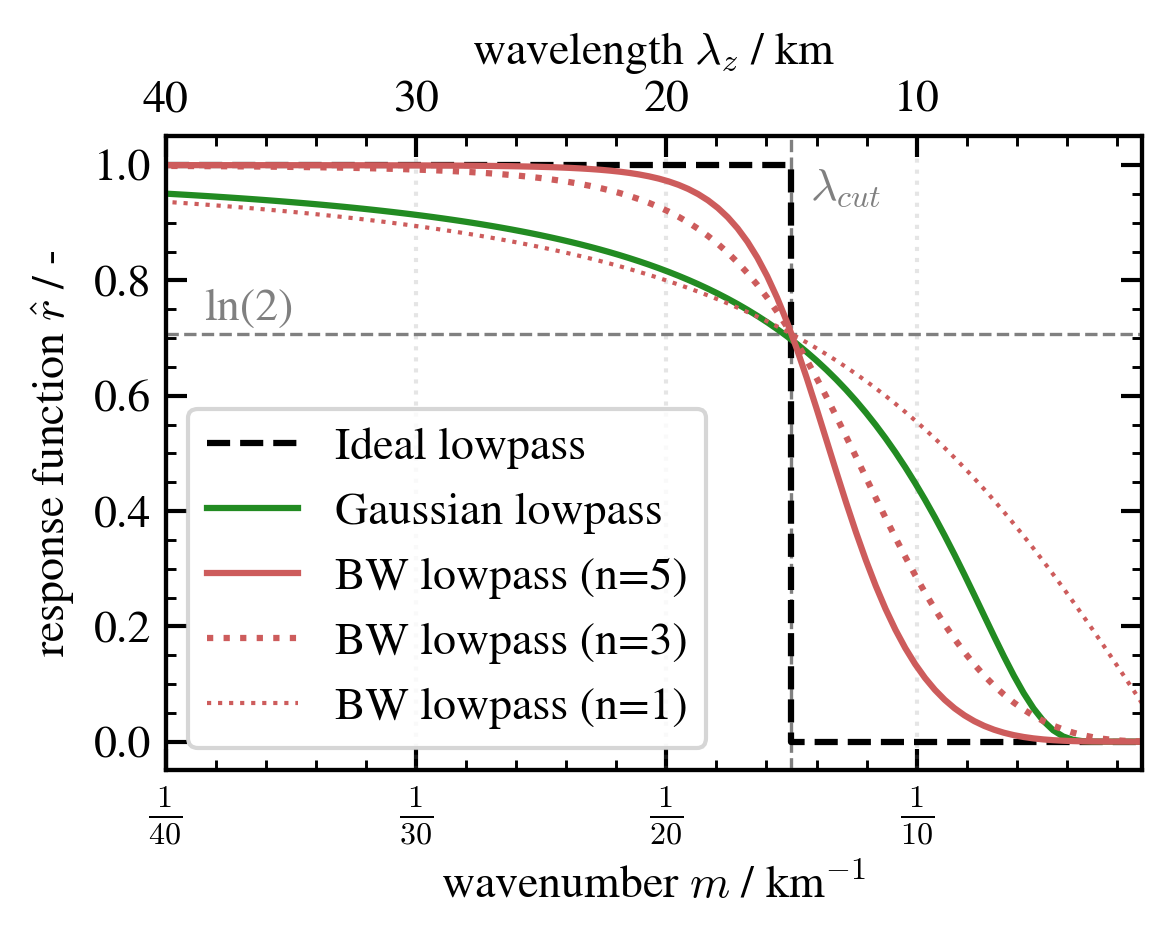
\includegraphics[width=0.55\textwidth]{figures_methods/filter_comparison.png}
    \caption{Shown are the response functions $\hat{r}_{lp}(\lambda_z)$ of the idealized lowpass filter (solid black line), the lowpass Gaussian filter (solid green line), the fifth order (solid red line), third order (dotted red line) and first order (thin dotted red line) lowpass Butterworth filter. The horizontal dashed grey line indicates the \SI{-3}{dB} level where a normalized signal is reduced to $\ln(2)$.}
    \label{fig:filter_comp}
    % and the $\frac{1}{e}$ level.
    % and the opposite of a highpass Butterworth filter (solid golden line)
\end{figure*}
%
\subsection*{Butterworth filter for separating perturbations and a background state}
To analyse time-height diagrams of temperature measurements by the Rayleigh lidar CORAL described in Section \ref{sec:coral}, we us a Butterworth filter as recommended by \textcite[]{ehard_evaluation_2015}. In many cases, this lidar dataset suffers from time gaps, so the absolute temperature measurements are filtered vertically to provide a more robust setup.
%  separate perturbations from a background state 

Again, we use a lowpass filter to obtain the temperature background and then subtract the background from the original dataset to gain the perturbations. The response function of the Butterworth lowpass filter is defined by 
\begin{equation}
    \hat{r}_{lp,bw}(\lambda_z) = \Biggl(1+\Bigl(\frac{\lambda_{cut}}{\lambda_{z}}\Bigr)^{2n}\Biggr)^{-\frac{1}{2}}
    \label{equ:butterworth_filter}
\end{equation}
with the order $n$. We utilize a fifth order ($n=5$) Butterworth filter as visualized Figure \ref{fig:filter_comp}. \textcite{butterworth_theory_1930} designed this filter such that its response function is relatively flat, which means low frequencies remain nearly unchanged and high frequencies are almost completely suppressed. For smaller values of $n$ the cutoff is less sharp or flat, but even a third order Butterworth filter is significantly flatter than a Gaussian filter. Figure \ref{fig:filter_comp} further emphasizes this flatter response function of the Butterworth filter for higher orders and in comparison to the Gaussian filter.

Again, the dataset is padded before the DFT as described for the Gaussian filter. Another interesting comparison between different filter methods, including a Gaussian and a Butterworth filter, is found in \textcite{krisch_superposition_2020}.

% For the following analysis the cutoff wavelength is defined as λcut = 15km, a value used in multiple studies (Baumgarten et al., 2017, Bramberger et al., 2017, Kaifler et al., 2017, Rapp et al., 2018a).
%
% However, if the Butterworth cutoff is extended to 30km, a non-negligible fraction of variance from tides, PWs, and seasonal oscillations leaks into the high-pass signal.

\section{Wavelet transform}
\label{sec:wavelet}
%
The wavelet transform is used for deriving horizontal and vertical wavelengths of GWs in the idealized numerical simulations described in Chapter \ref{sec:results3D}. Unlike the Fourier transform mentioned in the previous section, which analyses a signal purely in the frequency domain, the wavelet transform operates in the frequency and the spatial (or temporal) domain. Therefore, it provides information on the dominant scales (frequencies) and on their spatial distribution. This makes it a useful tool to determine GW scales at specific locations.\\

A comprehensive overview on the wavelet transform is given by \textcite{torrence_practical_1998}. We will briefly introduce the method by means of Figure \ref{fig:wavelet_example}. The vertical profile of potential temperature $\Theta'(z)$ in (a) is given on an equidistant grid with vertical resolution $\Delta z$ and the index $j=0,...,N-1$. Spatially localized waves, so-called wavelets, are the basis of a wavelet transform. We use the Morlet wavelet
\begin{equation}
    \psi(\eta)_0= \pi^{-\frac{1}{4}} {\rm e}^{i \omega_0 \eta}  {\rm e}^{-\frac{\eta^2}{2}}
    \label{equ:morlet}
\end{equation}
with the dimensionless location parameter $\eta$ and the nondimensional frequency $\omega_0$. The real and imaginary parts of $\psi(j')_0$ are plotted in grey in Figure \ref{fig:wavelet_example}a. We can now think of a wavelet transform in terms of moving the wavelet along the vertical axis (as indicated by the grey arrow in (a)) and constantly multiplying $\psi(j')_0$ with the $\Theta'(j')$ for each position $j$ of the wavelet. This process is then repeated for several scales of $\psi(j')_0$.\\ From a mathematical point of view, the wavelet transform of a discrete sequence $\Theta'(j')$ is defined as the convolution of $\Theta'(j')$ with a scaled and translated version of $\psi(j')_0$.
\begin{equation}
    W(s,j)=\sum_{j'=0}^{N-1} \Theta(j') \psi^{*}  \Biggl( \frac{(j'-j) \Delta z}{s}  \Biggr),
    \label{equ:wavelet_transform}
\end{equation}
where $s$ is the scale parameter and $\psi^{*}$ is the complex conjugate of the Morlet wavelet $\psi = \Bigl(\frac{\Delta z}{s} \Bigr)^{1/2} \psi_0$. The real wavelet coefficients $\left| W(s,j) \right|$ obtained for each scale $s$ and position $j$ of the wavelet can be visualized in a space-frequency plot similar to Figure \ref{fig:wavelet_example}b, which shows the distribution of the power spectrum across different scales (wavelengths or frequencies) and different vertical positions. In the example in Figure \ref{fig:wavelet_example}, the wavelet spectrum suggests that the most relevant wavelengths are approximately \SI{8}{\kilo\meter} and found around $z \approx \SI{50}{\kilo\meter}$. This coincides with the vertical profile $\Theta'(z)$ in (a). 

Although it is possible to calculate the wavelet transform using Equation \ref{equ:wavelet_transform}, it is considerably faster to do the calculations in Fourier space, where we can apply the wavelet transform for all $j$ at once. For a more detailed description we refer to \textcite{torrence_practical_1998}.\\
It is recommended to to choose $M$ different scales for the wavelet $\psi_0$ according to 
\begin{equation}
    s_m = s_0 2^{m \Delta m} \quad \textrm{with} \quad m = 0,1,...,M \quad \textrm{and} \quad M = \Delta m^{-1} \log_2(N \frac{\Delta m}{s_0}).    
\end{equation}
For the Morlet wavelet, a $\Delta m=0.5$ is the largest value that still provides an adequate sampling of the scale and $s_0$ should be chosen such that the equivalent Fourier period is approximately $2 \Delta z$.
% This value depends on the width of the wavelet function in spectral-space

\begin{figure*}[t]
    \centering
    \includegraphics[width=0.67\textwidth]{figures_methods/waveletAna_power_spectrum.png}
    \caption{Shown is an example of a vertical profile of potential temperature perturbations $\Theta'$ from an EULAG simulation in (a) and the corresponding wavelet power spectrum scaled by the variance $\sigma^2$ in (b). Grey lines in (a) illustrate the real (solid) and imaginary (dashed) parts of the Morlet-Wavelet introduced by \textcite{torrence_practical_1998}. The grey arrow indicates the position change of the wavelet for the wavelet transform. Hashed areas in (b) indicate the cone of influence and the green dashed line represents the \SI{95}{\percent} confidence level with respect to red noise (\cite[]{torrence_practical_1998}).}
    \label{fig:wavelet_example}
\end{figure*}
As in the context of the spectral filters (Section \ref{sec:spectral_filter}), the Fourier transformation assumes that the dataset is cyclic. Again, this leads to discontinuities and errors can occur at the beginning and end of the wavelet power spectrum. The hashed area in Figure \ref{fig:wavelet_example}b is the region of the wavelet spectrum in which these edge effects become important. It is called the cone of influence (COI).\\
The normalization of the wavelet power spectrum in (b) with the variance of the data $\sigma^2$ gives a measure of the power relative to white noise. In addition, the green dashed line in (b) indicates the \SI{95}{\percent} confidence level with respect to a red-noise background spectrum with lag-1 coefficient $\alpha=0.72$ (\cite{torrence_practical_1998}).

The 3D wave properties derived in Chapter \ref{sec:results3D} are based on one-dimensional wavelet transforms performed in each spatial dimension. The wavelength that corresponds to the maximum in the wavelet power spectrum is retained for each grid point of the dataset.

% For many geophysical phenomena, an appropriate background spectrum is either white noise (with a flat Fourier spectrum) or red noise (increasing power with decreasing frequency)
% confidence level with respect to red-noise background spectrum for α= 0.72

\section{CORAL temperature measurements} 
\label{sec:coral}
The COmpact Rayleigh Autonomous Lidar (CORAL) is a ground-based Rayleigh/Raman backscatter light detection and ranging (lidar) system that was developed and built by the German Aerospace Center (DLR). It is the first fully automatic middle atmosphere lidar that measures temperature in an altitude range from 15 to about \SI{90}{\kilo\meter} (\cite{kaifler_compact_2021}). CORAL does not have a daylight filter, so its operation is still limited to nighttime and clearsky conditions. However, its automatisation results in a $3-8$ times higher measurement cadence than any comparable human-operated lidar system. Since its installation in Río Grande, Argentina (53.79°S, 67.75°W) in November 2017, the lidar system CORAL provides time series of vertical temperature profiles at the world's strongest GW hotspot, the southern tip of South America (\cite{kaifler_compact_2021}).

The basic building blocks of a lidar are a transmitter and a receiver. In the case of CORAL, the transmitter is a diode-pumped pulsed Nd:YAG laser, which operates at \SI{1064}{nm} (\SI{532}{nm} after conversion to the second harmonic) with a pulse repetition rate of \SI{100}{Hz} and delivers \SI{120}{mJ} per pulse. These pulses of intense laser light are shot in the atmosphere where they are subject to Rayleigh scattering on air molecules.\\
The receiver is two-part and involves the telescope and the receiver unit. The telescope comprises a parabolic mirror with a diameter of \SI{630}{mm} and an aperture of f/2.45 resulting in a \SI{361}{\micro rad} field of view. It focuses the collected light into an optical fiber which is positioned in the mirror's focal point and connected to the receiver box. In the receiver box, the beam is collimated and spectrally divided using a dichroic mirror which separates the elastic scattering at \SI{532}{nm} wavelength and the nitrogen rotational Raman scattering at approximately \SI{608}{nm} wavelength. The beam containing the elastic scattering is further split into three beams (low, mid and far channel) to increase the dynamic range of the detection. The detector of the far channel sees \SI{92}{\percent}, the mid channel receives \SI{7.4}{\percent} and only \SI{0.6}{\percent} of the light reaches the low channel. For further details on the technical setup of CORAL, we refer to \textcite{kaifler_compact_2021}.
%
% Automatic tracking of the laser beam is realized by the implementation of the conical scan method. 
% In order to increase the dynamic range of the detection, the beam containing the elastic scattering is further split into three beams with a splitting ratio of approximately 92.0 : 7.4 : 0.6, i.e., the detector of the far channel sees 92 % of the light, while only 0.6 % of the light reaches the low channel.
\begin{figure*}[t]
    \centering
    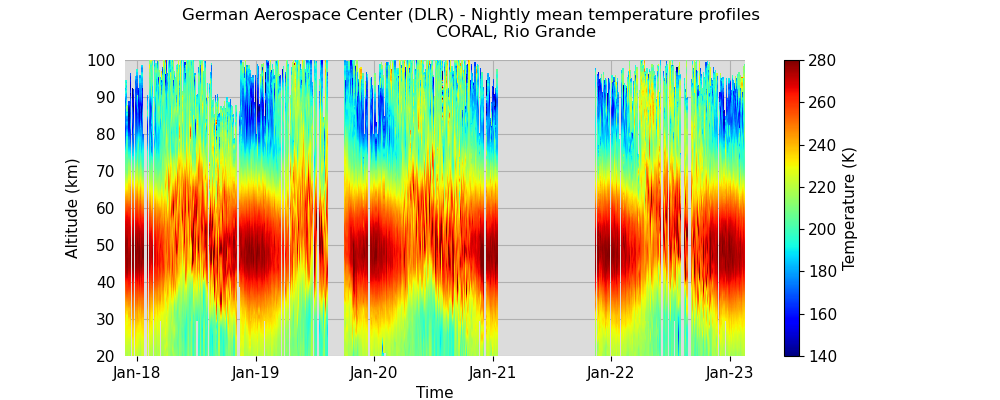
\includegraphics[width=0.99\textwidth]{figures_methods/coral_nightly_means.png}
    \caption{Time-height diagram of temperature $T$, which comprises all nightly mean temperature profiles obtained by CORAL from November 2017 until today (February 2023). Grey areas indicate times without measurements. The large data gaps in the fall of 2019 and in 2021 are due to technical issues with the instrument.}
    \label{fig:coral_dataset}
\end{figure*}

CORAL's standard temperature data product has a \SI{900}{\meter} vertical and \SI{20}{\minute} temporal resolution. Figure \ref{fig:coral_dataset} provides a general overview on the available dataset since CORAL's installation at the end of 2017. Technical issues led to significant data gaps from mid-August until mid-November 2019 and from January until November 2021. During the remaining periods, CORAL operated whenever conditions permitted observations resulting in measurements on 2 out of 3 nights on average (\cite[]{kaifler_compact_2021}). A comprehensive analysis of CORAL's measurements is found in \textcite{reichert_highcadence_2021} and \textcite{reichert_characterization_2022} and individual observations are visualized \href{http://container.kaifler.net/coral/index.php}{here}\footnote[1]{http://container.kaifler.net/coral/index.php}. 

%
% Comment on temperature retrieval

\section{ERA5 reanalysis dataset}
\label{sec:era5}
%
In Chapter \ref{cha:lidar} we use the ERA5 reanalysis introduced by \textcite[]{hersbach_et_al_era5_2020} for two case studies in the context of GW observations by the ground-based lidar CORAL at the southern tip of South America.\\
The ERA5 reanalysis is based on the Integrated Forecasting System (IFS) by the European Centre for Medium-Range Weather Forecasts (ECMWF). More specifically, it is based on the IFS model cycle 41r2 with a horizontal resolution of roughly \SI{9}{\kilo\meter} which was operational in 2016. The resulting ERA5 product is upscaled to a grid spacing of 0.25° or about \SI{31}{\kilo\meter}.\\
One part of the ERA5 analysis includes the analysis of upper stratosphere temperature perturbations and comparing them to measurements of CORAL. Therefore, it should be noted that upper levels in the IFS and ERA5 data are affected by vertical sponge layers, which dampen resolved upward propagating GWs to prevent wave reflection at the model top.\\
The stratospheric sponge starts at \SI{10}{hPa} ($\approx \SI{30}{\kilo\meter}$) and applies a rather weak fourth-order hyperdiffusion on the vertical component of vorticity, horizontal divergence and temperature. In addition, a much stronger mesospheric sponge of order 1 acts on the horizontal divergence above \SI{1}{hPa} ($\approx \SI{45}{\kilo\meter}$).

For the analysis in Chapter \ref{cha:lidar}, we used the ERA5 reanalysis on model levels (\cite[]{hersbach_era5_2018}) and on pressure levels (\cite{hersbach_era5_2018-1}) publicly available through the Climate Data Store of the Copernicus Climate Change Service.

% Copernicus Climate Change Service (C3S) Climate Data Store (CDS)
% ERA5 thus benefits from a decade of developments in model physics, core dynamics and data assimilation.
% and height of dynamical tropopause (2 PVU level)
% - maybe also comment on observational filter of satellite measurments from with figure from Hindley